%%%%%%%%%%%%%%%%%%%%%%%%%%%%%%%%%%%%%%%%%%%%%%%%%%%%%%%%%%%%%%%%%%%%%%%%
% Plantilla TFG/TFM
% Escuela Politécnica Superior de la Universidad de Alicante
% Realizado por: Jose Manuel Requena Plens
% Contacto: info@jmrplens.com / Telegram:@jmrplens
%%%%%%%%%%%%%%%%%%%%%%%%%%%%%%%%%%%%%%%%%%%%%%%%%%%%%%%%%%%%%%%%%%%%%%%%
\chapter{Resultados}
\label{resultados}
En este apartado usaré comparaciones en gráficas para ver claramente las ventajas y/o inconvenientes de algunas decisiones que he tomado durante el desarrollo de este proyecto.

\section{Optimización de caché}
Como he mencionado en el desarrollo, el motor \gls{ecs} está pensado para ser ``cache-friendly''. Esto quiere decir que la memoria del programa se organiza de tal manera que optimiza la caché. Esto sucede, como ya he comentado, porque la caché lee streams de memoria, y no solo un dato. Por lo tanto, merece la pena tener los datos que vayamos a utilizar en el juego ordenados en memoria, de esta manera el juego podrá realizar más acciones por frame, debido a que la velocidad de un acceso a memoria en caché es, aproximadamente, 200 veces más rápida que un acceso a memoria RAM.
\\
Por lo tanto, he simplificado un ejemplo con el cual demostrar que el orden en el que se lee la memoria es importante. El siguiente código es una matriz, la cual se lee primero de manera "cache-friendly", y después no.
\begin{lstlisting}[style=C-color, caption={Caché optimizada vs sin optimizar.},label=cache-optimization]
size_t bench_optimized(size_t v[][width], size_t times) {
	size_t result = 0;
	
	for(size_t i=0; i<times; ++i) {
		for (size_t j = 0; j < height; ++j) 
			for (size_t k = 0; k < width; ++k)
				result += v[j][k];
	}
	
	return result;
}
size_t bench_unoptimized(size_t v[][width], size_t times) {
	size_t result = 0;
	
	for(size_t i=0; i<times; ++i) {
		for (size_t k = 0; k < width; ++k) 
			for (size_t j = 0; j < height; ++j) 
				result += v[j][k];
	}
	
	return result;
}
\end{lstlisting}

La diferencia en ambos métodos está en los dos for anidados. Una vez tenemos los dos métodos, procedo a hacer una comparación, y el resultado es el de la siguiente figura:
\begin{figure}[ht]
	\centering
	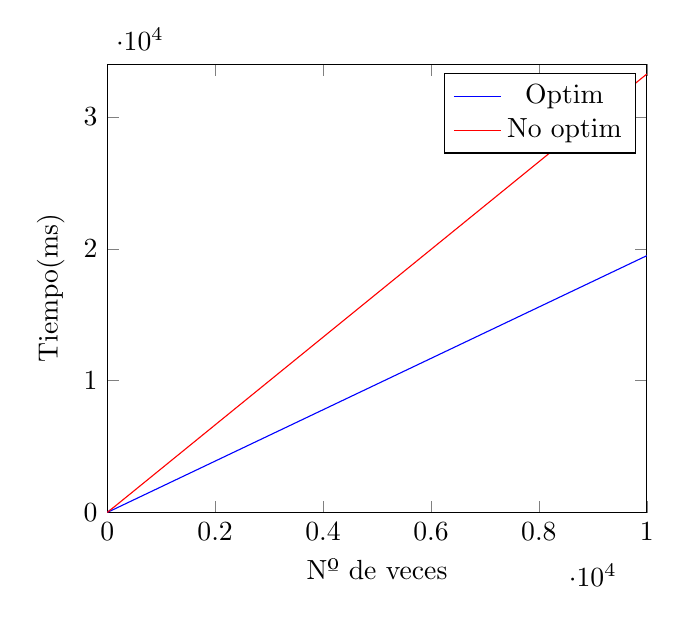
\begin{tikzpicture}
		\begin{axis}
			[ymin=0,ymax=34000, 
			xmin=0,xmax=10000, 
			ylabel= Tiempo(ms), 
			xlabel= Nº de veces] 
			\addplot+[smooth, mark=none] coordinates 
			{(1,2) (10,32) (100,196) (1000,1949) (10000,19479)};
			\addplot+[smooth, mark=none] coordinates
			{(1,3) (10,34) (100,332) (1000,3317) (10000,33256)};
			\legend{Optim, No optim}
		\end{axis}
	\end{tikzpicture}
	\caption{Comparación de optimización vs sin optimización.}
\end{figure}

El resultado es claro, en cualquier caso acceder a la memoria de forma desordenada es un 50\% más costoso en este test. Por lo que la deducción es que hay que intentar mantener la memoria ordenada para una mayor eficiencia del programa. 
\\
Un apunte final que me veo obligado a hacer es que, tanto con el compilador de clang++, como el de g++, no hay que usar el flag ``-O3''. De ser así, al ser un test tan simple, el compilador es capaz de optimizar el código máquina y los resultados de ambos test son los mismos.

\section{Aprendizaje aleatorio vs Backpropagation}
Como quiero comparar las ventajas de usar Backpropagation, lo voy a hacer contra el algoritmo más sencillo, el que tenía inicialmente, que es el algoritmo aleatorio explicado en la figura \ref{Algoritmo aleatorio}. El problema que se tratará de resolver con el algoritmo es el de la XOR, y la arquitectura que va a tener la red neuronal es dos neuronas de entrada, una capa oculta con tres neuronas, y una neurona de salida que dice si la entrada ha producido verdadero o falso. 
\\
Como vemos en la siguiente figura, la linea roja representa el error que tiene la red cada 10 iteraciones, y la linea azul representa cómo va mejorando el error cuando el algoritmo se guarda el mejor resultado hasta el momento. Hay que tener en cuenta que, al ser cuatro soluciones las que tiene que dar (falso y falso, falso y verdadero, verdadero y falso, verdadero y verdadero), pero hay que representar el verdadero y el false numéricamente para calcular el error de la red, un error menor al 25\% significa que ha ajustado los pesos de la red para que los cuatro casos coincidan con la solución.
\begin{figure}[ht]
	\centering
	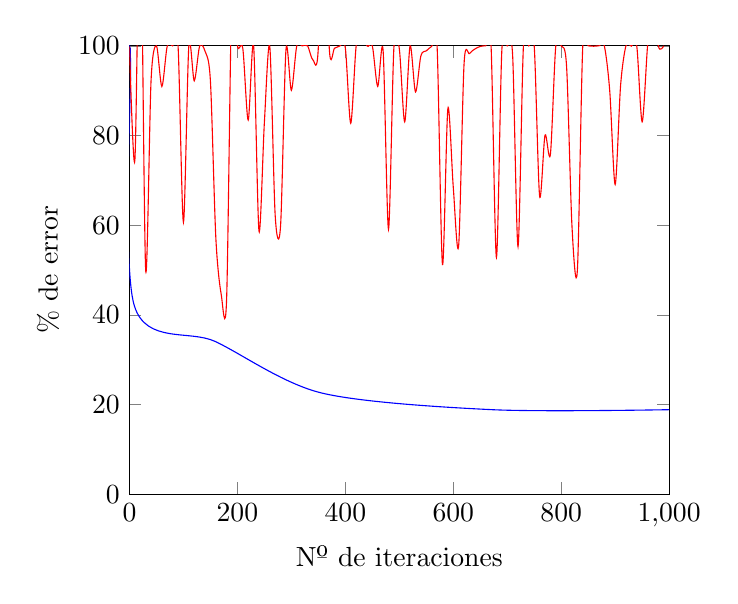
\begin{tikzpicture}
		\begin{axis}
			[ymin=0,ymax=100, 
			xmin=0,xmax=1000, 
			ylabel= \% de error, 
			xlabel= Nº de iteraciones] 
			\addplot+[smooth, mark=none] coordinates 
			{(0,101.14) (0,99.8454) (1,97.5228) (2,95.9093) (9,42.0106) (159,34.0462) (355,22.5898) (672,18.837) (1000,18.837)};
			\addplot+[smooth, mark=none] coordinates
			{(0,99.8454) (10,74.5026) (20,133.048) (30,50.0229) (40,92.3021) (50,100.001) (60,90.9467) (70,99.9676) (80,99.999) (90,99.994) (100,60.6559) (110,99.9855) (120,92.1943) (130,99.9257) (140,98.7933) (150,92.1119) (160,57.2305) (170,44.5407) (180,43.5673) (190,113.788) (200,100) (210,99.4142) (220,83.4381) (230,100.071) (240,58.6687) (250,82.9632) (260,99.8364) (270,62.1711) (280,59.9009) (290,99.1347) (300,90.076) (310,100) (320,99.984) (330,99.9887) (340,96.8439) (350,99.8101) (360,147.47) (370,100) (380,99.4627) (390,99.9865) (400,99.528) (410,82.7241) (420,99.9637) (430,104.989) (440,99.9984) (450,99.988) (460,90.9419) (470,98.9157) (480,59.0847) (490,99.6393) (500,99.3816) (510,83.033) (520,100) (530,89.7185) (540,97.7787) (550,98.865) (560,99.872) (570,99.9869) (580,51.2202) (590,85.9898) (600,68.4817) (610,55.4502) (620,95.9602) (630,98.2658) (640,99.2841) (650,99.8679) (660,99.999) (670,99.9999) (680,52.8244) (690,98.9702) (700,99.9932) (710,97.9063) (720,55.2218) (730,99.942) (740,99.9992) (750,99.9678) (760,66.4945) (770,80.0553) (780,75.8166) (790,100.012) (800,99.9916) (810,95.3353) (820,59.7116) (830,49.9807) (840,99.9995) (850,99.9919) (860,99.9067) (870,99.9991) (880,99.9417) (890,89.8568) (900,69.0741) (910,91.0636) (920,99.9952) (930,99.9321) (940,100) (950,83.0578) (960,99.9856) (970,112.699) (980,99.9977) (990,100)};
		\end{axis}
	\end{tikzpicture}
	\caption{Resultados del aprendizaje con un algoritmo aleatorio.}
\end{figure}

Otro dato interesante a conocer es en qué iteración el algoritmo encuentra una solución válida para resolver la XOR. El algoritmo itera 1000 veces. Después de ejecutar el algoritmo durante 10.000 intentos, llego a la conclusión empírica de que el algoritmo encuentra una solución en la iteración 354.16 de media, siempre que lo encuentra. Sin embargo, hay un 19.83\% de las veces que el algoritmo aleatorio no es capaz de encontrar la solución. 
\\
Y no sólo vamos a fijarnos en el número de iteraciones que necesita el algoritmo, sino también en el tiempo, para después poder comparar con cuánto tiempo tarda contra Backpropagation. El algoritmo aleatorio tarda 12 segundos, en entrenar 10.000 veces en mi máquina con optimizaciones, lo que quiere decir que de media tarda 0.0012 segundos en resolver el problema.

En la siguiente figura veremos, con una estructura de la red neuronal equivalente (dos neuronas de entrada, una capa oculta con tres neuronas, y una neurona de salida). Como veremos a continuación, el número de iteraciones que hay que hacer para alcanzar una solución válida es mayor.

\begin{figure}[ht]
	\centering
	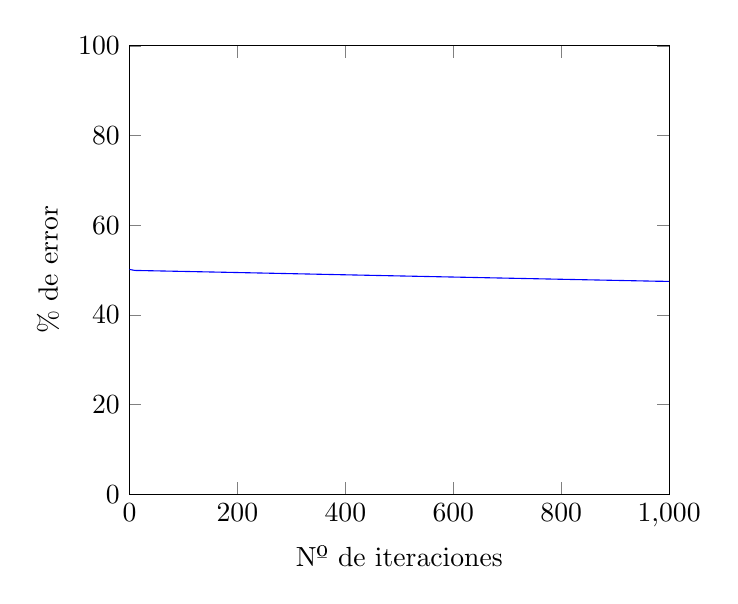
\begin{tikzpicture}
		\begin{axis}
			[ymin=0,ymax=100, 
			xmin=0,xmax=1000, 
			ylabel= \% de error, 
			xlabel= Nº de iteraciones] 
			\addplot+[smooth, mark=none] coordinates 
			{(0,50.1247) (10,49.8995) (20,49.8748) (30,49.8501) (40,49.8255) (50,49.8009) (60,49.7764) (70,49.7518) (80,49.7272) (90,49.7025) (100,49.6779) (110,49.6531) (120,49.6284) (130,49.6036) (140,49.5787) (150,49.5538) (160,49.5289) (170,49.5039) (180,49.4789) (190,49.4538) (200,49.4287) (210,49.4035) (220,49.3784) (230,49.3532) (240,49.3279) (250,49.3027) (260,49.2774) (270,49.2521) (280,49.2268) (290,49.2015) (300,49.1762) (310,49.1509) (320,49.1256) (330,49.1002) (340,49.0749) (350,49.0496) (360,49.0243) (370,48.999) (380,48.9737) (390,48.9485) (400,48.9232) (410,48.898) (420,48.8727) (430,48.8475) (440,48.8223) (450,48.7971) (460,48.772) (470,48.7468) (480,48.7217) (490,48.6966) (500,48.6715) (510,48.6464) (520,48.6214) (530,48.5963) (540,48.5713) (550,48.5463) (560,48.5213) (570,48.4964) (580,48.4715) (590,48.4465) (600,48.4216) (610,48.3967) (620,48.3719) (630,48.347) (640,48.3222) (650,48.2974) (660,48.2726) (670,48.2478) (680,48.223) (690,48.1982) (700,48.1735) (710,48.1487) (720,48.124) (730,48.0993) (740,48.0746) (750,48.0499) (760,48.0252) (770,48.0006) (780,47.9759) (790,47.9513) (800,47.9266) (810,47.902) (820,47.8774) (830,47.8527) (840,47.8281) (850,47.8035) (860,47.7789) (870,47.7543) (880,47.7297) (890,47.7052) (900,47.6806) (910,47.656) (920,47.6314) (930,47.6069) (940,47.5823) (950,47.5577) (960,47.5332) (970,47.5086) (980,47.4841) (1000,47.4595)};
		\end{axis}
	\end{tikzpicture}
	\caption{Resultados del aprendizaje con el algoritmo Backpropagation.}
\end{figure}

De los 10.000 intentos de que el algoritmo solucione el problema en 1000 iteraciones, sólo se consigue el 1.4\% de las veces, a diferencia del 80,17\% que conseguía el algoritmo aleatorio. Mientras que el tiempo que tarda el algoritmo de Backpropagation es equivalente, 12 segundos. Por lo tanto, hay que subir el número de iteraciones que hace. Con 10000, Backpropagation tarda 1 minuto y 54 segundos y acierta el 33.43\% de las veces, y con 100000 tarda 17 minutos y 13 segundos y acierta el 76.51\% de las veces. En este último caso con mayor porcentaje de acierto, de media acierta en la iteración 21421.6, esto tiene sentido ya que con 10000 el porcentaje de acierto era muy bajo, por lo que, de media, la solución se encuentra en una iteración superior.
\\
Esto quiere decir que, para el problema de la XOR en concreto, el algoritmo aleatorio resuelve antes respecto a número de iteraciones y respecto al tiempo. Pero, ¿a qué se debe esto? Un motivo puede ser que debido al bajo número de parámetros libres que tiene el sistema (en este caso los pesos de la red neuronal), un algoritmo aleatorio sea suficiente para resolver el problema, pero cuanto más crezca el sistema, más improbable será encontrar una solución de forma aleatoria. En este sentido, la conclusión es que ambos algoritmos son igual de rápidos, pero para sistemas pequeños el algoritmo aleatorio aprenderá antes.

La siguiente gráfica muestra, ya que Backpropagation tiene un parámetro para ajustar la velocidad de aprendizaje, una comparación entre diferentes posibles valores del mismo. 
\begin{figure}[ht]
	\centering
	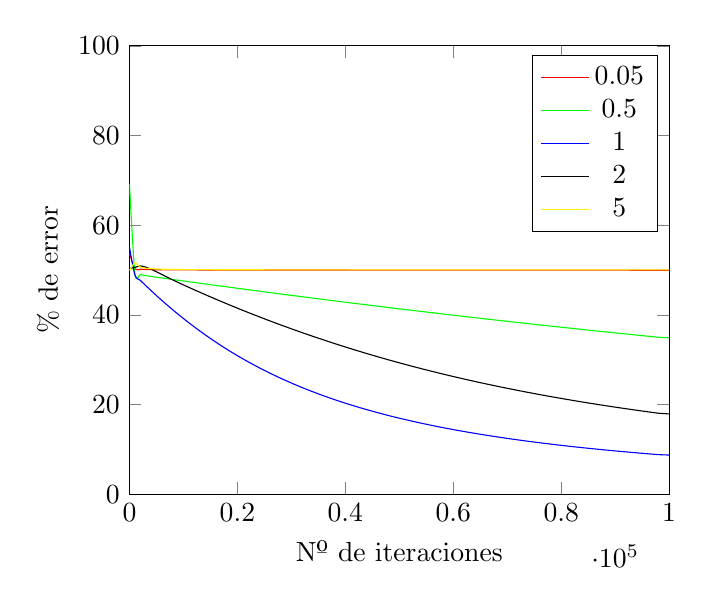
\begin{tikzpicture}
		\begin{axis}
			[ymin=0,ymax=100, 
			xmin=0,xmax=100000, 
			ylabel= \% de error, 
			xlabel= Nº de iteraciones] 
			\addplot+[smooth, mark=none, color=red] coordinates 
			{(0,53.7617) (1000,50.2511) (2000,50.1684) (3000,50.1148) (4000,50.0797) (5000,50.0565) (6000,50.0407) (7000,50.0298) (8000,50.022) (9000,50.0163) (10000,50.0121) (11000,50.0088) (12000,50.0062) (13000,50.004) (14000,50.0023) (15000,50.0008) (16000,49.9994) (17000,49.9983) (18000,49.9972) (19000,49.9963) (20000,49.9954) (21000,49.9945) (22000,49.9937) (23000,49.993) (24000,49.9922) (25000,49.9915) (26000,49.9908) (27000,49.9901) (28000,49.9894) (29000,49.9888) (30000,49.9881) (31000,49.9875) (32000,49.9868) (33000,49.9862) (34000,49.9855) (35000,49.9849) (36000,49.9843) (37000,49.9836) (38000,49.983) (39000,49.9824) (40000,49.9818) (41000,49.9811) (42000,49.9805) (43000,49.9799) (44000,49.9793) (45000,49.9786) (46000,49.978) (47000,49.9774) (48000,49.9768) (49000,49.9762) (50000,49.9756) (51000,49.9749) (52000,49.9743) (53000,49.9737) (54000,49.9731) (55000,49.9725) (56000,49.9718) (57000,49.9712) (58000,49.9706) (59000,49.97) (60000,49.9694) (61000,49.9688) (62000,49.9682) (63000,49.9675) (64000,49.9669) (65000,49.9663) (66000,49.9657) (67000,49.9651) (68000,49.9645) (69000,49.9638) (70000,49.9632) (71000,49.9626) (72000,49.962) (73000,49.9614) (74000,49.9608) (75000,49.9602) (76000,49.9595) (77000,49.9589) (78000,49.9583) (79000,49.9577) (80000,49.9571) (81000,49.9565) (82000,49.9558) (83000,49.9552) (84000,49.9546) (85000,49.954) (86000,49.9534) (87000,49.9528) (88000,49.9522) (89000,49.9515) (90000,49.9509) (91000,49.9503) (92000,49.9497) (93000,49.9491) (94000,49.9485) (95000,49.9478) (96000,49.9472) (97000,49.9466) (98000,49.946) (100000,49.9454) };
			\addplot+[smooth, mark=none, color=green] coordinates 
			{(0,69.1556) (1000,49.3072) (2000,48.9651) (3000,48.7441) (4000,48.5577) (5000,48.3828) (6000,48.2123) (7000,48.0439) (8000,47.8767) (9000,47.7103) (10000,47.5446) (11000,47.3794) (12000,47.2147) (13000,47.0505) (14000,46.8869) (15000,46.7237) (16000,46.561) (17000,46.3988) (18000,46.2371) (19000,46.0759) (20000,45.9152) (21000,45.755) (22000,45.5953) (23000,45.4361) (24000,45.2774) (25000,45.1192) (26000,44.9615) (27000,44.8044) (28000,44.6477) (29000,44.4916) (30000,44.336) (31000,44.1809) (32000,44.0263) (33000,43.8722) (34000,43.7187) (35000,43.5657) (36000,43.4132) (37000,43.2612) (38000,43.1098) (39000,42.9589) (40000,42.8085) (41000,42.6586) (42000,42.5093) (43000,42.3605) (44000,42.2122) (45000,42.0645) (46000,41.9173) (47000,41.7706) (48000,41.6245) (49000,41.4789) (50000,41.3338) (51000,41.1893) (52000,41.0453) (53000,40.9018) (54000,40.7588) (55000,40.6164) (56000,40.4745) (57000,40.3332) (58000,40.1924) (59000,40.0521) (60000,39.9123) (61000,39.7731) (62000,39.6344) (63000,39.4963) (64000,39.3586) (65000,39.2216) (66000,39.085) (67000,38.9489) (68000,38.8134) (69000,38.6785) (70000,38.544) (71000,38.4101) (72000,38.2767) (73000,38.1438) (74000,38.0115) (75000,37.8796) (76000,37.7483) (77000,37.6176) (78000,37.4873) (79000,37.3576) (80000,37.2284) (81000,37.0997) (82000,36.9715) (83000,36.8438) (84000,36.7167) (85000,36.5901) (86000,36.464) (87000,36.3384) (88000,36.2133) (89000,36.0887) (90000,35.9646) (91000,35.8411) (92000,35.718) (93000,35.5955) (94000,35.4735) (95000,35.3519) (96000,35.2309) (97000,35.1104) (98000,34.9904) (100000,34.8708) };
			\addplot+[smooth, mark=none, color=blue] coordinates 
			{(0,55.0694) (1000,48.8877) (2000,47.694) (3000,46.5299) (4000,45.3939) (5000,44.2861) (6000,43.2065) (7000,42.1549) (8000,41.1312) (9000,40.1351) (10000,39.1664) (11000,38.2246) (12000,37.3094) (13000,36.4204) (14000,35.5571) (15000,34.719) (16000,33.9055) (17000,33.1161) (18000,32.3503) (19000,31.6074) (20000,30.8869) (21000,30.1882) (22000,29.5107) (23000,28.8538) (24000,28.2169) (25000,27.5993) (26000,27.0006) (27000,26.4201) (28000,25.8573) (29000,25.3116) (30000,24.7824) (31000,24.2692) (32000,23.7715) (33000,23.2888) (34000,22.8206) (35000,22.3663) (36000,21.9255) (37000,21.4978) (38000,21.0827) (39000,20.6798) (40000,20.2886) (41000,19.9087) (42000,19.5399) (43000,19.1815) (44000,18.8334) (45000,18.4952) (46000,18.1665) (47000,17.8469) (48000,17.5363) (49000,17.2342) (50000,16.9404) (51000,16.6546) (52000,16.3765) (53000,16.1059) (54000,15.8424) (55000,15.586) (56000,15.3363) (57000,15.093) (58000,14.8561) (59000,14.6253) (60000,14.4003) (61000,14.181) (62000,13.9672) (63000,13.7588) (64000,13.5555) (65000,13.3571) (66000,13.1636) (67000,12.9748) (68000,12.7905) (69000,12.6106) (70000,12.4349) (71000,12.2633) (72000,12.0957) (73000,11.932) (74000,11.772) (75000,11.6157) (76000,11.4629) (77000,11.3135) (78000,11.1674) (79000,11.0245) (80000,10.8847) (81000,10.748) (82000,10.6141) (83000,10.4832) (84000,10.355) (85000,10.2295) (86000,10.1067) (87000,9.98636) (88000,9.86852) (89000,9.75307) (90000,9.63996) (91000,9.52912) (92000,9.4205) (93000,9.31402) (94000,9.20963) (95000,9.10728) (96000,9.00692) (97000,8.90848) (98000,8.81192) (100000,8.71719) };
			\addplot+[smooth, mark=none, color=black] coordinates 
			{(0,50.3149) (1000,50.5792) (2000,50.9022) (3000,50.638) (4000,50.1671) (5000,49.5938) (6000,48.9877) (7000,48.3868) (8000,47.8018) (9000,47.2315) (10000,46.6726) (11000,46.123) (12000,45.5813) (13000,45.0468) (14000,44.5189) (15000,43.9975) (16000,43.4823) (17000,42.9731) (18000,42.4699) (19000,41.9725) (20000,41.4809) (21000,40.9951) (22000,40.515) (23000,40.0406) (24000,39.5719) (25000,39.1088) (26000,38.6513) (27000,38.1994) (28000,37.7531) (29000,37.3123) (30000,36.8771) (31000,36.4473) (32000,36.0231) (33000,35.6042) (34000,35.1909) (35000,34.7829) (36000,34.3803) (37000,33.9831) (38000,33.5911) (39000,33.2045) (40000,32.8231) (41000,32.4469) (42000,32.0759) (43000,31.7101) (44000,31.3493) (45000,30.9936) (46000,30.643) (47000,30.2973) (48000,29.9565) (49000,29.6206) (50000,29.2896) (51000,28.9633) (52000,28.6418) (53000,28.325) (54000,28.0128) (55000,27.7052) (56000,27.4021) (57000,27.1036) (58000,26.8094) (59000,26.5197) (60000,26.2342) (61000,25.953) (62000,25.6761) (63000,25.4033) (64000,25.1346) (65000,24.8699) (66000,24.6092) (67000,24.3525) (68000,24.0996) (69000,23.8506) (70000,23.6053) (71000,23.3637) (72000,23.1258) (73000,22.8915) (74000,22.6607) (75000,22.4334) (76000,22.2095) (77000,21.9891) (78000,21.7719) (79000,21.558) (80000,21.3474) (81000,21.1399) (82000,20.9355) (83000,20.7342) (84000,20.5359) (85000,20.3406) (86000,20.1482) (87000,19.9586) (88000,19.7719) (89000,19.5879) (90000,19.4067) (91000,19.2281) (92000,19.0522) (93000,18.8788) (94000,18.708) (95000,18.5397) (96000,18.3739) (97000,18.2104) (98000,18.0493) (100000,17.8906) };
			\addplot+[smooth, mark=none, color=yellow] coordinates 
			{(0,49.9271) (1000,51.5363) (2000,50.6184) (3000,50.3785) (4000,50.2706) (5000,50.2099) (6000,50.171) (7000,50.1441) (8000,50.1244) (9000,50.1094) (10000,50.0976) (11000,50.088) (12000,50.0802) (13000,50.0736) (14000,50.068) (15000,50.0631) (16000,50.059) (17000,50.0553) (18000,50.052) (19000,50.0491) (20000,50.0466) (21000,50.0442) (22000,50.0421) (23000,50.0402) (24000,50.0384) (25000,50.0368) (26000,50.0353) (27000,50.034) (28000,50.0327) (29000,50.0315) (30000,50.0304) (31000,50.0294) (32000,50.0284) (33000,50.0276) (34000,50.0267) (35000,50.0259) (36000,50.0252) (37000,50.0245) (38000,50.0238) (39000,50.0232) (40000,50.0226) (41000,50.022) (42000,50.0215) (43000,50.0209) (44000,50.0204) (45000,50.02) (46000,50.0195) (47000,50.0191) (48000,50.0187) (49000,50.0183) (50000,50.0179) (51000,50.0175) (52000,50.0172) (53000,50.0169) (54000,50.0165) (55000,50.0162) (56000,50.0159) (57000,50.0156) (58000,50.0154) (59000,50.0151) (60000,50.0148) (61000,50.0146) (62000,50.0144) (63000,50.0141) (64000,50.0139) (65000,50.0137) (66000,50.0135) (67000,50.0133) (68000,50.0131) (69000,50.0129) (70000,50.0127) (71000,50.0125) (72000,50.0123) (73000,50.0121) (74000,50.012) (75000,50.0118) (76000,50.0116) (77000,50.0115) (78000,50.0113) (79000,50.0112) (80000,50.011) (81000,50.0109) (82000,50.0108) (83000,50.0106) (84000,50.0105) (85000,50.0104) (86000,50.0103) (87000,50.0101) (88000,50.01) (89000,50.0099) (90000,50.0098) (91000,50.0097) (92000,50.0096) (93000,50.0095) (94000,50.0094) (95000,50.0093) (96000,50.0092) (97000,50.0091) (98000,50.009) (100000,50.0089) };
			\legend{0.05, 0.5, 1, 2, 5}
		\end{axis}
	\end{tikzpicture}
	\caption{Resultados del aprendizaje con el algoritmo Backpropagation, según el learning rate.}
\end{figure}

Se aprecia que ratios de aprendizaje extremadamente bajos y extremadamente altos hacen que la red no aprenda bien, por diferentes motivos. No se puede decir un ratio que sea común para todos los problemas, por eso en el juego dejo experimentar al usuario con distintos ratios para que encuentre el mejor. 

\section{Backpropagation en el juego}
\todo{Mostrar cómo aprende la red neuronal con diferentes valores dentro del juego}